\subsection{Pixel Operations}

\begin{frame}{Region copy}
  \begin{itemize}
  \item Requirements for all pixel operations:
    \begin{itemize}
    \item The source and destination must use the same pixel format
    \item Must be converted before any operation otherwise
    \end{itemize}
  \item Most basic operation on pixels: copying a region
    \begin{itemize}
    \item Also known as bit blit or BITBLT (in reference to the hardware opcode)
    \end{itemize}
  \item Implemented as a line-per-line copy (maximum memory-contiguous block)
  \item Overwriting destination memory with source memory
    \begin{itemize}
    \item Copies within the same image are not always safe!
    \item Destination must not overlap source
    \end{itemize}
  \end{itemize}
\end{frame}

\begin{frame}{Alpha blending}
  \begin{itemize}
  \item Compositing multiple alpha-enabled pixel sources into a single result
    \begin{itemize}
    \item Simplest case: aggregating sources with z-ordered stacking
    \item Equation for A over B (with \(\alpha\) the alpha and \(C\) the color component value):
    \end{itemize}
\[
C_o = \frac{C_a \alpha_a + C_b \alpha_b \left(1 - \alpha_a\right)}{\alpha_a + \alpha_b \left(1 - \alpha_a\right)}
\]
  \item With alpha available, many more operations become possible
    \begin{itemize}
    \item Shapes can be used as masks, with logic operators
    \item Formalized by Porter and Duff in 1984
    \end{itemize}
  \end{itemize}
  \begin{center}
  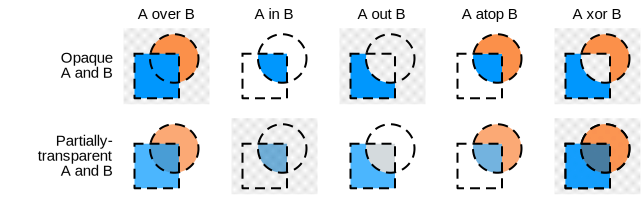
\includegraphics[width=0.5\textwidth]{slides/graphics-theory-pixel-operations/porter-duff-compositing.pdf}
  \end{center}
\end{frame}

\begin{frame}{Color-keying}
  \begin{itemize}
  \item Color-keying (or chroma-keying): replacing given colors with alpha
  \item Specified with color ranges (3 RGB ranges)
  \item Pixels either within or outside of the range are made transparent
  \item Used in conjunction with alpha blending
  \item The famous video green-screen method uses color-keying
  \end{itemize}
  \begin{center}
  \includegraphics[width=0.5\textwidth]{slides/graphics-theory-pixel-operations/chroma-key-blender.jpg}\\
  \textit{\small Color-keying implemented in Blender}
  \end{center}
\end{frame}

\begin{frame}{Scaling and interpolation}
  \begin{itemize}
  \item Scaling is a resizing operation on a pixel picture
    \begin{itemize}
    \item Involves a scaling factor (integer or real)
    \item Values are resampled with a new resolution
    \item Requires reconstructing the original signal
    \end{itemize}
  \item Implemented with some form of interpolation:
    \begin{itemize}
    \item nearest-neighbor: uses the nearest pixel value from the source
\[
x_{source} = x_{destination} \div scale
\]
  \item bilinear interpolation: sub-pixel linear weighting of neighbor colors
  \item bicubic interpolation: smooth spline sub-pixel fitting with neighbor colors
    \end{itemize}
  \item Sub-pixel methods provide better visual results
  \item Down-sampling:
    \begin{itemize}
    \item Reduces the maximum image frequency
    \item Can cause aliasing: high frequencies need to be removed
    \end{itemize}
  \end{itemize}
\end{frame}

\begin{frame}{Linear filtering and convolution}
  \begin{itemize}
  \item Filtering is a transformation of each pixel based on its neighbors
  \item The pixel output value is a linear sum of weighted neighboring input values
\[
o_{x,y} = \alpha_0 i_{x,y} + \alpha_1 i_{x-1,y} + \alpha_2 i_{x+1,y} + ...
\]
  \item Weighting coefficients are represented in a 2D matrix: the \textbf{filter kernel}
    \begin{itemize}
    \item Comes with \(2n + 1\) columns and \(2m + 1\) rows
    \item The coefficients are applied to each input pixel and its neighbors
    \item The element at the kernel center weights the current input pixel
    \end{itemize}
  \item Corresponds to a \textbf{convolution} operation between pixels and the filter kernel
  \item High computational cost (optimizations are implemented)
  \item Allows many applications for 2D signal processing
  \end{itemize}
\end{frame}

\begin{frame}{Linear filtering and convolution (illustrated)}
  \begin{center}
  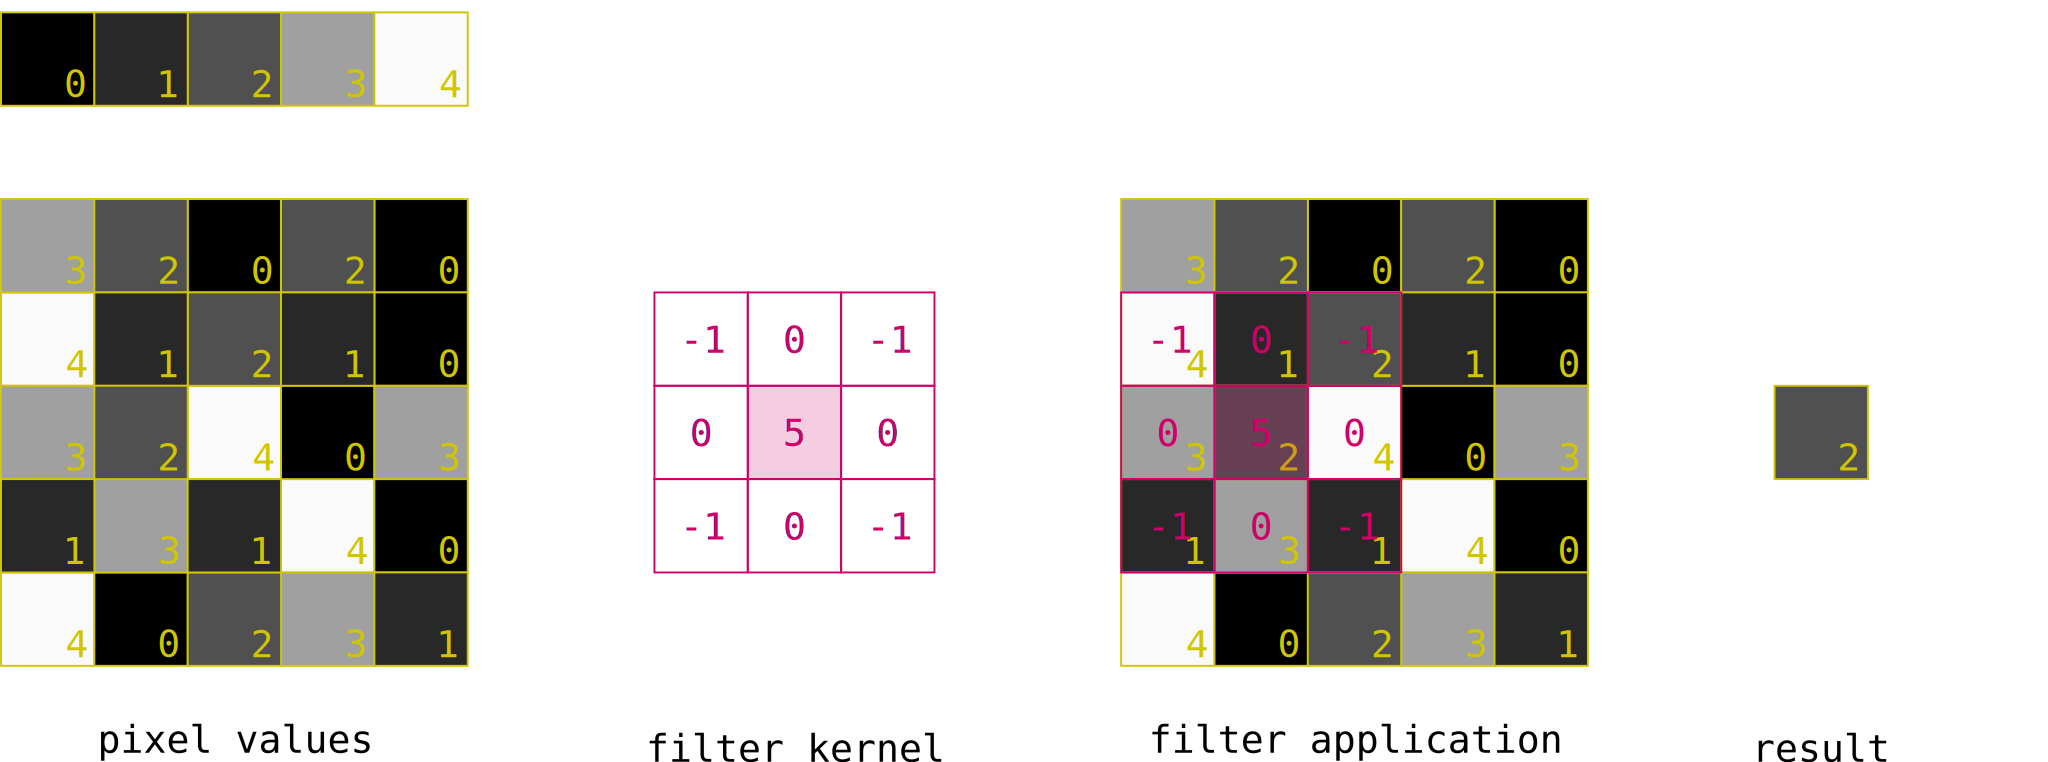
\includegraphics[width=0.7\textwidth]{slides/graphics-theory-pixel-operations/linear-filtering.pdf}\\
  \textit{\small Linear filtering in application}
\[
g(x,y)= \omega *f(x,y)=\sum_{s=-n}^n{\sum_{t=-m}^m{ \omega (s,t)f(x-s,y-t)}}
\]
  \textit{\small Bi-dimensional convolution operation on \(f\) with the \(\omega\) kernel}
  \end{center}
\end{frame}

\begin{frame}{Blur filters}
  \begin{itemize}
  \item Blurring is a common example of linear filtering
  \item Corresponds to a low-pass filter
    \begin{itemize}
    \item Removes high frequencies from the picture (details)
    \item Good fit for pre-scaling anti-aliasing
    \end{itemize}
\begin{minipage}[b]{0.45\textwidth}
  \item Implemented with different algorithms:
    \vspace{-1.5em}
    \begin{itemize}
    \item Box blur: rough but easy to optimize
\[
\frac{1}{9}
\left[
\begin{matrix}
1 & 1 & 1 \\
1 & 1 & 1 \\
1 & 1 & 1
\end{matrix}
\right]
\]
    \end{itemize}
\end{minipage}
\begin{minipage}[b]{0.45\textwidth}
    \begin{itemize}
    \item Gaussian blur: reference smooth blur
\[
\frac{1}{16}
\left[
\begin{matrix}
1 & 2 & 1 \\
2 & 4 & 2 \\
1 & 2 & 1
\end{matrix}
\right]
\]
    \end{itemize}
    \end{minipage}
  \item A repeated box blur converges towards a Gaussian one (central-limit theorem)
  \end{itemize}
\end{frame}

\begin{frame}{Dithering}
  \begin{itemize}
  \item Reducing the color depth can lead to visually-unpleasant results
    \begin{itemize}
    \item Corresponds to color-space down-sampling
    \item Increases color quantization error
    \end{itemize}
  \item Floyd–Steinberg dithering is a method for improving quality with low depth
  \item Quantization error is evaluated and distributed to neighboring pixels
  \item Used in hardware display engines and the GIF file format
  \end{itemize}~\\

  \begin{minipage}[t]{0.25\textwidth}
    \centering
    \includegraphics[width=0.9\textwidth]{slides/graphics-theory-pixel-operations/cat-depth-initial.png}\\
    \textit{\small Cat at initial depth}
  \end{minipage}
  \hfill
  \begin{minipage}[t]{0.25\textwidth}
    \centering
    \includegraphics[width=0.9\textwidth]{slides/graphics-theory-pixel-operations/cat-depth-low.png}\\
    \textit{\small Cat at reduced depth without dithering}
  \end{minipage}
  \hfill
  \begin{minipage}[t]{0.25\textwidth}
    \centering
    \includegraphics[width=0.9\textwidth]{slides/graphics-theory-pixel-operations/cat-depth-dither.png}\\
    \textit{\small Cat at reduced depth with dithering}
  \end{minipage}
\end{frame}

\begin{frame}{Graphics theory online references}
  \small
  \begin{itemize}
  \item Wikipedia (\url{https://en.wikipedia.org/}):
    \begin{itemize}
    \item \href{https://en.wikipedia.org/wiki/Color_model}{Color model}
    \item \href{https://en.wikipedia.org/wiki/Color_depth}{Color depth}
    \item \href{https://en.wikipedia.org/wiki/YCbCr}{YCbCr}
    \item \href{https://en.wikipedia.org/wiki/Chroma_subsampling}{Chroma subsampling}
    \item \href{https://en.wikipedia.org/wiki/Nyquist–Shannon_sampling_theorem}{Nyquist–Shannon sampling theorem}
    \item \href{https://en.wikipedia.org/wiki/Spatial_anti-aliasing}{Spatial anti-aliasing}
    \item \href{https://en.wikipedia.org/wiki/Aliasing}{Aliasing}
    \item \href{https://en.wikipedia.org/wiki/Line_drawing_algorithm}{Line drawing algorithm}
    \item \href{https://en.wikipedia.org/wiki/Parametric_equation}{Parametric equation}
    \item \href{https://en.wikipedia.org/wiki/Alpha_compositing}{Alpha compositing}
    \item \href{https://en.wikipedia.org/wiki/Image_scaling}{Image scaling}
    \item \href{https://en.wikipedia.org/wiki/Kernel_(image_processing)}{Kernel (image processing)}
    \end{itemize}
  \item \url{http://ssp.impulsetrain.com/porterduff.html}
  \item \url{https://magcius.github.io/xplain/article/regions.html}
  \item \url{https://magcius.github.io/xplain/article/rast1.html}
  \end{itemize}
\end{frame}

\begin{frame}{Graphics theory illustrations attributions}
  \small
  \begin{itemize}
  \item \href{https://commons.wikimedia.org/wiki/File:2017-12-28_Leipzig,_34c3,_Fairy_Dust_(freddy2001).jpg}{34C3 Fairy Dust: Freddy2001, CC BY-SA 3.0}
  \item \href{https://commons.wikimedia.org/wiki/File:View_from_the_Window_at_Le_Gras,_Joseph_Nic\%C3\%A9phore_Ni\%C3\%A9pce.jpg}{Point de vue du Gras: Joseph Nicéphore Niépce, public domain}
  \item \href{https://commons.wikimedia.org/wiki/File:Pinball_Dot_Matrix_Display_-_Demolition_Man.JPG}{Pinball Dot Matrix Display: ElHeineken, CC BY 3.0}
  \item \href{https://commons.wikimedia.org/wiki/File:Soderledskyrkan_brick_wall.jpg}{Soderledskyrkan brick wall: Xauxa, CC BY-SA 3.0}
  \item \href{https://commons.wikimedia.org/wiki/File:AliasingSines.svg}{Aliasing Sines: Moxfyre, CC BY-SA 3.0}
  \item \href{https://commons.wikimedia.org/wiki/File:Moire_pattern_of_bricks.jpg}{Moiré pattern of bricks: Colin M.L. Burnett, CC BY-SA 3.0}
  \item \href{https://commons.wikimedia.org/wiki/File:Moire_pattern_of_bricks_small.jpg}{Moiré Pattern at Gardham Gap: Roger Gilbertson, CC BY-SA 2.0}
  \item \href{https://commons.wikimedia.org/wiki/File:RGBCube_a.svg}{RGB cube: Datumizer, CC BY-SA 4.0}
  \item \href{https://commons.wikimedia.org/wiki/File:Pair_of_Merops_apiaster_feeding.jpg}{Pair of Merops apiaster feeding: Pierre Dalous, CC BY-SA 3.0}
  \end{itemize}
\end{frame}

\begin{frame}{Graphics theory illustrations attributions}
  \small
  \begin{itemize}
  \item \href{https://commons.wikimedia.org/wiki/File:Hsl-hsv_models_b.svg}{Hsl-hsv models: Datumizer, CC BY-SA 3.0}
  \item \href{https://commons.wikimedia.org/wiki/File:Barns_grand_tetons.jpg}{Barns grand tetons: Jon Sullivan, public domain}
  \item \href{https://commons.wikimedia.org/wiki/File:Top-left_triangle_rasterization_rule.gif}{Top-left triangle rasterization rule: Drummyfish, CC0 1.0}
  \item \href{https://commons.wikimedia.org/wiki/File:Line_scan-conversion.svg}{Line scan-conversion: Phrood, CC BY-SA 3.0}
  \item \href{https://commons.wikimedia.org/wiki/File:Alpha_compositing.svg}{Alpha compositing: Prometeusm, Wereon, public domain}
  \item \href{https://commons.wikimedia.org/wiki/File:Blender3D_com_key_chroma.jpg}{Blender3D com key chroma: Toni Grappa, Blender Foundation, CC BY-2.5}
  \item \href{https://en.wikipedia.org/wiki/File:Dithering_example_dithered_web_palette.png}{Dithering example: Jamelan, CC BY-SA 3.0}
  \end{itemize}
\end{frame}
